%%%%%%%%%%%%%%%%%%%%%%%%%%%%%%%%%%%%%%%%%
%
% CMPT 435
% Lab Zero
%
%%%%%%%%%%%%%%%%%%%%%%%%%%%%%%%%%%%%%%%%%

%%%%%%%%%%%%%%%%%%%%%%%%%%%%%%%%%%%%%%%%%
% Short Sectioned Assignment
% LaTeX Template
% Version 1.0 (5/5/12)
%
% This template has been downloaded from: http://www.LaTeXTemplates.com
% Original author: % Frits Wenneker (http://www.howtotex.com)
% License: CC BY-NC-SA 3.0 (http://creativecommons.org/licenses/by-nc-sa/3.0/)
% Modified by Alan G. Labouseur  - alan@labouseur.com
%
%%%%%%%%%%%%%%%%%%%%%%%%%%%%%%%%%%%%%%%%%

%----------------------------------------------------------------------------------------
%	PACKAGES AND OTHER DOCUMENT CONFIGURATIONS
%----------------------------------------------------------------------------------------

\documentclass[letterpaper, 10pt]{article} 

\usepackage[english]{babel} % English language/hyphenation
\usepackage{graphicx}
\usepackage{xcolor}
\graphicspath{ {./images/} }
\usepackage[lined,linesnumbered,commentsnumbered]{algorithm2e}
\usepackage{listings}

% Lstlistings configuration
\definecolor{codegreen}{rgb}{0,0.6,0}
\definecolor{codegray}{rgb}{0.5,0.5,0.5}
\definecolor{codepurple}{rgb}{0.58,0,0.82}
\definecolor{backcolour}{rgb}{0.95,0.95,0.92}

\lstdefinestyle{mystyle}{
    backgroundcolor=\color{backcolour},   
    commentstyle=\color{codegreen},
    keywordstyle=\color{magenta},
    numberstyle=\tiny\color{codegray},
    stringstyle=\color{codepurple},
    basicstyle=\ttfamily\footnotesize,
    breakatwhitespace=false,         
    breaklines=true,                 
    captionpos=b,                    
    keepspaces=true,                 
    numbers=left,                    
    numbersep=5pt,                  
    showspaces=false,                
    showstringspaces=false,
    showtabs=false,                  
    tabsize=2
}

\lstset{style=mystyle}
\lstset{language=Java}

\usepackage{fancyhdr} % Custom headers and footers
\pagestyle{fancyplain} % Makes all pages in the document conform to the custom headers and footers
\usepackage{lastpage}
\usepackage{wasysym}
\usepackage{url}

% Set up for minted package. It had some bugs so I decided to only keep lstlistings.
% \usepackage{minted}
% \makeatletter
% \newlength\minted@belowskip
% \define@key{minted@opt}{belowskip}[\@topsepadd]
% {\setlength{\minted@belowskip}{#1}}

% \def\minted@endparenv{%
%   \addpenalty\@endparpenalty\addvspace\minted@belowskip\@endpetrue}
% \def\FV@EndList{%
%   \FV@ListProcessLastLine
%   \FV@EndListFrame
%   \minted@endparenv
%   \endgroup
%   \@endpetrue}
% \makeatother
% \newminted{java}{linenos=true, belowskip=3cm}

\fancyhead{} % No page header - if you want one, create it in the same way as the footers below
\fancyfoot[L]{} % Empty left footer
\fancyfoot[C]{page \thepage\ of \pageref{LastPage}} % Page numbering for center footer
\fancyfoot[R]{}

\renewcommand{\headrulewidth}{0pt} % Remove header underlines
\renewcommand{\footrulewidth}{0pt} % Remove footer underlines
\setlength{\headheight}{13.6pt} % Customize the height of the header

%----------------------------------------------------------------------------------------
%	TITLE SECTION
%----------------------------------------------------------------------------------------

\newcommand{\horrule}[1]{\rule{\linewidth}{#1}} % Create horizontal rule command with 1 argument of height

\title{	
   \normalfont \normalsize 
   \textsc{CMPT 435 - Fall 2021 - Dr. Labouseur} \\[10pt] % Header stuff.
   \horrule{0.5pt} \\[0.25cm] 	% Top horizontal rule
   \huge Assignment Four - Graphs and Binary Trees \\     	    % Assignment title
   \horrule{0.5pt} \\[0.25cm] 	% Bottom horizontal rule
}

\author{Augusto Gonzalez-Bonorino \\ \normalsize augusto.gonzalezbonorino1@marist.edu}

\date{\normalsize\today} 	% Today's date.

\begin{document}

\maketitle % Print the title

%----------------------------------------------------------------------------------------
%   CONTENT SECTION
%----------------------------------------------------------------------------------------

% - -- -  - -- -  - -- -  -

\section{Description of program}

The program I will discuss in the following sections is concerned with the implementation of a Binary Tree class and, arguably one of the most important mathematical objects, Graphs which were discovered by Leonhard Euler in 1752. This document is organized in the following manner: 1) Description of the program; 2) Explanation and implementation of a Vertex; 3) Explanation and implementation of a Graph in java; 4) Manipulating and Displaying the Graph; 5) Explanation and implementation of Binary Tree; 6) Walk-through over Main class; 7) Results and conclusion; 8) Further thoughts.
\begin{center}
    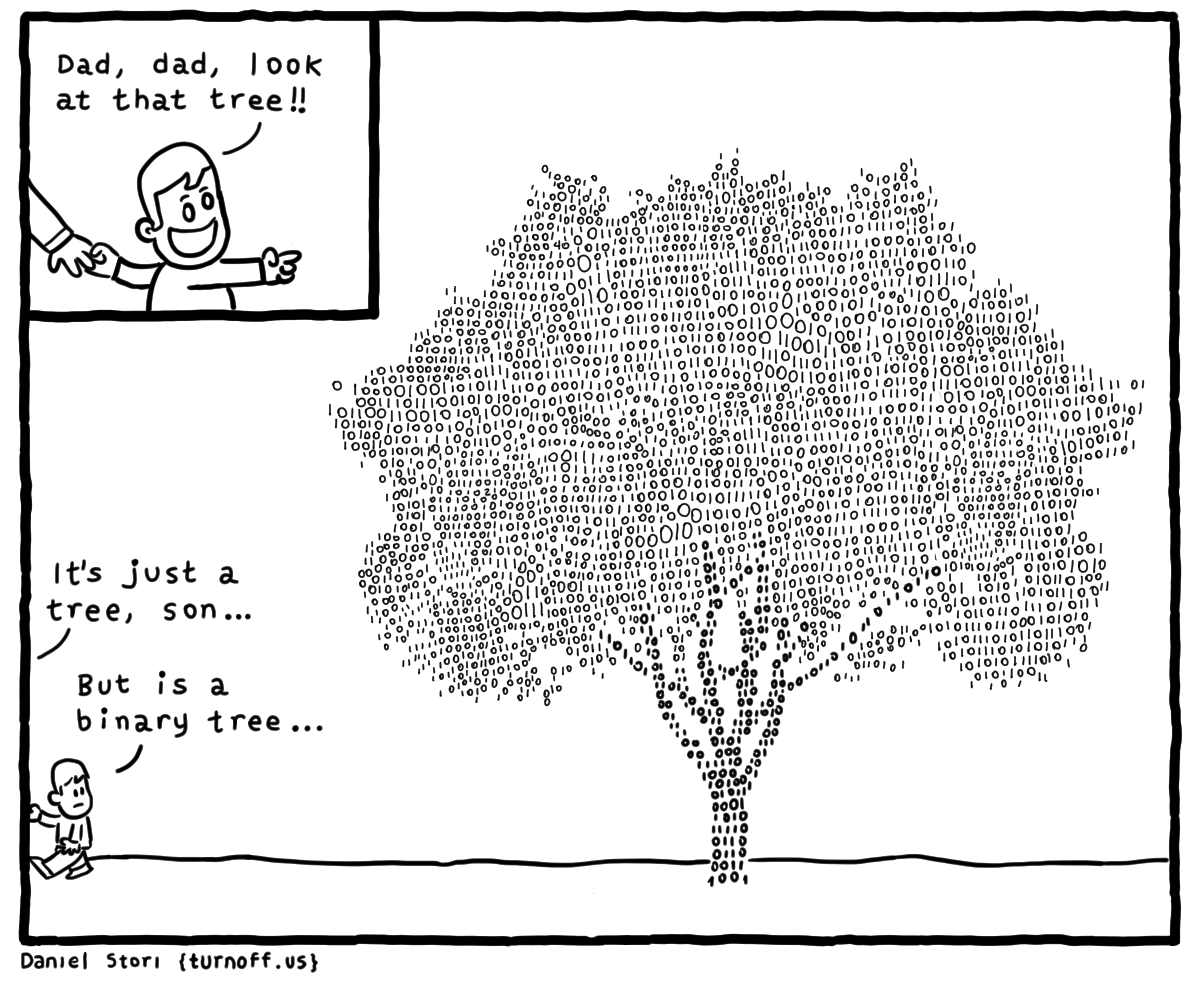
\includegraphics[scale=0.18]{images/binary-tree.png}
\end{center}
\\
\section{Vertex}
\\
Graphs are composed of nodes, vertices, that can be connected to other vertices by edges. The vertex is the object who holds the data we are working with - an integer corresponding to the vertex's id in this case - a collection of neighbours (vertices connected by an edge and one-hop distance apart) and a "switch" to check if it was processed or not to avoid double checking vertices. Here is how my implementation in Java looks like:
\\
\begin{lstlisting}
public class VertexGonzalezBonorino {

	private int myId;
	
	private ArrayList<VertexGonzalezBonorino> myNeighbours;
	
	private VertexGonzalezBonorino myNext;
	
	private boolean processed;
	
	// constructor
	
	public VertexGonzalezBonorino(int newId)
		{
			
			myId = newId;
			myNext = null;
			processed = false;
			myNeighbours = new ArrayList<>();
			
		} // VertexGonzalezBonorino
\end{lstlisting}
\\
Note that I store the neighbours of each vertex on an ArrayList which, even though is a bit slower, allows me to freely modify the size of the list unlike regular Arrays. Moreover, \textit{myNext} is nothing else than a pointer which will be used to create a linked list of the nodes of the graph that will allow us to traverse it with a pair of algorithms. Keep reading to find out which algorithms. Besides the usual getters and setters I have defined 5 methods that are worth analyzing. Here is my code:
\\
\begin{lstlisting}
public ArrayList<VertexGonzalezBonorino> getNeighbours()
		{
			return myNeighbours;
			
		} // getNeighbours
	
	public void addNeighbour(VertexGonzalezBonorino neighbour)
		{
			myNeighbours.add(neighbour);
			
		} // addNeighbour
	
	public boolean isProcessed()
		{
			return processed;
			
		} // isProcessed
	
	public void process()
		{
			processed = true;
			
		} // process
	
	public void unprocess()
		{
			processed = false;
			
		} // unprocess
	

    public void addEdge(VertexGonzalezBonorino newNeighbour)
	    {
	        myNeighbours.add(newNeighbour);
	        
	    } // addEdge
\end{lstlisting}
\\
The first two methods in the listing above give me the capability of accessing the vertex's neighbours and adding new ones. The function \textit{isProcessed()} returns if the vertex has been visited (i.e. processed) previously, the following function processes the vertex and the third function unprocesses it, a useful helper method I included to implement multiple graphs sequentially. Lastly, the method \textit{addEdge} connects to nodes to each other (both ways because we are implementing an undirected graph) by adding the input vertex to the current vertex's list of neighbours.
\\
\section{Undirected Graphs}
\\
A graph is a set of vertices and a collection of edges that each connect a pair of vertices. Undirected graphs are a special type of Graph for which the relations between pairs of vertices are symmetric, meaning that the edges have no direction and thus a connection between two vertices flows both ways. Graphs have applications all around, from modelling neural and social networks to communication or mechanical circuits. Therefore, it is a great thing that we have learnt how to implement and leverage such a powerful data structure. An undirected graph can be displayed in multiple ways, for this program we will employ the following three: Adjacency list, Matrix form and as a linked list. Before discussing these methods in more detail, let's take a look at the building blocks of a  Graph.
\\
\begin{lstlisting}
public class GraphGonzalezBonorino {
	
	private int numVertices;
	
	public ArrayList<VertexGonzalezBonorino> myVertices;
	
	/**
	 * Constructor
	 */
	public GraphGonzalezBonorino()
		{
			myVertices = new ArrayList<>();
			
		} // GraphGonzalezBonorino
	
	/**
	 * Add vertex to graph given vertex object and id
	 * @param newVertex
	 * @param id
	 */
	public void addVertex(int id)
		{	
		
			VertexGonzalezBonorino newVertex = new VertexGonzalezBonorino(id);
			myVertices.add(newVertex);
			
			numVertices++;
			
		} // addVertex
\end{lstlisting}
\\
The main component to observe is the ArrayList that contains the vertices in the Graph. It is a list of Vertex objects which correspond to each of the nodes in the Graph. I also opted for initializing a variable to keep track of the number of vertices which, even though it does not have much functionality for this project, I believe might be useful if we want to keep track of the size of our Graph. lastly, the \textit{addVertex} method, as the name suggests, simply adds a new Vertex to our graph by appending it to our \textit{myVertices} ArrayList.

Now that we have the skeleton of our Graph and a way of adding vertices, we need a method to populate a graph given a list of commands. This will be useful for this particular project because we must read the instructions to create each graph from a text file. Each instruction is a String with the instruction and the id to assign to that vertex. Thus, as I will explain when we look at the Main class, we can store the instructions in a list of Strings and populate our graph based on those commands. Here is my method to populate our graph:
\\
\begin{lstlisting}
public void populateGraph(ArrayList<String> list)
	{

        //iterate through arrayList
        for(int i = 0; i < list.size(); i++)
        {
            //if line is empty or a comment, print it out
            if(list.get(i).equals("") || list.get(i).substring(0, 2).equals("--"))
            {
                System.out.println(list.get(i));
            }

            //if line wants us to add vertex...
            else if(list.get(i).contains("vertex"))
            {
                //take the last string, convert to an int and add a vertex with this id
                int id = Integer.parseInt(list.get(i).substring(list.get(i).lastIndexOf(" ") + 1));
                
                addVertex(id);

            }

            //if line wants us to add an edge...
            else if(list.get(i).contains("edge"))
            {
                //first id is first string after last instance of the letter 'e', until before the '-', convert to an int
                int id1 = Integer.parseInt(list.get(i).substring(list.get(i).lastIndexOf("e") + 2,
                        list.get(i).indexOf("-") - 1));
                //second id is from instance of '-' till end of string, convert to int
                int id2 = Integer.parseInt(list.get(i).substring(list.get(i).indexOf("-") + 2));

                //if the first node id is a 0, we take the id's as they are
                if(myVertices.get(0).getId() == 0)
                {
                	myVertices.get(id1).addEdge(myVertices.get(id2));
                	myVertices.get(id2).addEdge(myVertices.get(id1));
                }

                //if the first node is not a 0 (it will be 1), we need to subtract one
                // as ArrayLists start at 0 but our id is 1
                else 
                {
                	myVertices.get(id1 - 1).addEdge(myVertices.get(id2 - 1));
                	myVertices.get(id2 - 1).addEdge(myVertices.get(id1 - 1));
                }

            }
            
        } // for loop
        
    } // populateGraph
\end{lstlisting}
\\
It may look complicated, maybe even intimidating at first, but fear not because all we are doing here is parsing the text file to identify the instruction and the ids of the respective vertices. First, we look at the first line in the list of Strings we receive as input and check if it is a comment (characterized by a double hyphen "--") or a blank line. If so, we print it out to offer the user a description of the graph that will be implemented. Next, we check if we are being told to add a vertex or to add edges between vertices, by checking if the respective sub-string is found in the current String, and execute it. Now, adding a vertex is straightforward but adding an edge not so much so I it will be beneficial to dive a little deeper. First we parse the String to extract the ids specified in the instruction. Then, if the we are looking at the vertex with id 0 we simply connect it to the vertex with \textit{id2}. If it is not the first vertex, we must account for the index count that commences at 0 by subtracting 1 from the given indices. Voila! We have a fresh graph we can now play around with. Let's take a look at some of the methods we have implemented.
\\
\section{Displaying the Graph}
\\
As previously mentioned, we will implement three distinct methods for displaying the contents of our graph: Adjacency List, Adjacency Matrix and Linked List. An adjacency list is a function that maps each vertex to its neighbours. There are many ways in which it can be implemented such as using a Hash map, for example. I opted for implementing it in a way that I found more intuitive and easier to implement given my lack of experience with Java libraries. Let's take a look at the code first and then I will walk the reader through each component:
\\
\begin{lstlisting}
public void printAdjacencyList(GraphGonzalezBonorino graph)
	    {
	        //if first node starts at 1...
	        if(graph.myVertices.get(0).getId() == 1) 
		        {
		            //iterate through nodes
		            for (int i = 0; i < graph.myVertices.size(); i++) 
			            {
			                //print out i + 1 (since i is 0 but graph starts at  1) and print out the neighbors
			                System.out.print("[" + (i + 1) + "] ");
			                for (int j = 0; j < graph.myVertices.get(i).getNeighbours().size(); j++) 
				                {
				                    System.out.print(graph.myVertices.get(i).getNeighbours().get(j).getId() + " ");
				                    
				                } // inner for loop
			                
			                System.out.println();
			                
			            } // outer for loop
		            
		        } // if
	        
	        //else (graph starts at 0)
	        else
		        {
		            //same thing but we can print i directly
		            for (int i = 0; i < graph.myVertices.size(); i++) 
			            {
			                System.out.print("[" + i + "] ");
			                for (int j = 0; j < graph.myVertices.get(i).getNeighbours().size(); j++) 
				                {
				                    System.out.print(graph.myVertices.get(i).getNeighbours().get(j).getId() + " ");
				                    
				                } // inner for loop
			                
			                System.out.println();
			                
			            } // outer for loop
		            
		        } // else
	        
	    } // printAdjacencyList
\end{lstlisting}
\\
I consider two possible cases: If the vertex id equals 1 or if it equals 0 (zero). Recall that Java employs indices starting at 0, instead of 1 as in mathematics. Thus, if the vertex id is one we must take this into account by simply adding 1 to each id. This is the purpose of the if statement. Nevertheless, if the vertex's id equals 0 then we do not need to alter the value of the index. The algorithm to print out the Adjacency list is equivalent in both cases. First, we iterate over each vertex in the graph. Second, print out its id inside brackets. Finally, iterate over the neighbours if the current vertex and print their respective ids on the same line.

The second way of displaying the contents of our Graph is an Adjacency matrix, which is simply a square matrix containing 0s and 1s where 1 represents a connection between two vertices (i.e. they are neighbours). So, how does this look like in Java? Let's take a look at it.
\\
\begin{lstlisting}
    /**
     * Method to print the Matrix representation of the graph
     * @param GraphGonzalezBonorino object
     */
    public void printMatrix(GraphGonzalezBonorino graph)
	    {
	        int[][] matrix = new int[graph.myVertices.size()][graph.myVertices.size()];
	
	        //iterate through rows of matrix
	        for(int i = 0; i <graph.myVertices.size(); i++)
	        {
	            //iterate through columns of matrix
	            for(int j = 0; j < graph.myVertices.size(); j++)
		            {
		                //iterate through neighbors list
		                for(int k = 0; k < graph.myVertices.get(i).getNeighbours().size(); k++)
			                {
			                    //if first node starts at 0...
			                    if(graph.myVertices.get(0).getId() == 0)
				                    {
				                        //we check neighbor id directly to j and if they are equal, set matrix[i][j] to 1
				                        if(graph.myVertices.get(i).getNeighbours().get(k).getId() == j)
					                        {
					                            matrix[i][j] = 1;
					                            break;
					                            
					                        } // if
				                        
				                    } // if
			                    
			                   
			                    else
				                    {
				                        //we check neighbor id to j + 1 because matrices start at 0 while our graph starts at 1
				                        if(graph.myVertices.get(i).getNeighbours().get(k).getId() == j + 1)
					                        {
					                            matrix[i][j] = 1;
					                            break;
					                            
					                        } // if
				                        
				                    } // else
			
			                    matrix[i][j] = 0;
			                    
			                } // third loop
		
		            } // second loop
	            
	        } // first loop
	        
	        //print out matrix
	        for(int i = 0; i < graph.myVertices.size(); i++)
		        {
		            for(int j = 0; j < graph.myVertices.size(); j++)
			            {
			                System.out.print(matrix[i][j] + " ");
			                
			            } // inner for loop
		            
		            System.out.println();
		            
		        } // outer for loop
	        
	    } // printMatrix
\end{lstlisting}
\\
First, we initialize a matrix of dimensions equal to the size of the graph (which is equal to its number of vertices). Then, we perform an $n^2$ operation to iterate through each row and column. Next, we look at each vertex in the graph and get its neighbours. Here is where the magic happens. We want to append a 1 to the matrix at every cell that ``links" two vertices. For this, we check if the id of the neighbours of the current vertex equals the id of any of the vertices in the columns. If they are equal, append a 1 otherwise append a 0. Note that we must account for Java's zero index, just like we did for Adjacency List. This might be a bit overwhelming, it was for me, thus I believe it will be beneficial to illustrate the aforementioned idea with a simple example. 
\\
\begin{center}
    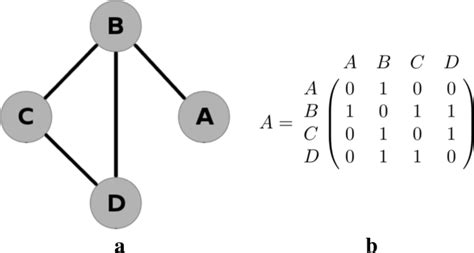
\includegraphics[scale=0.5]{images/adjMatrix.jpg}
\end{center}
\\
A 4x4 matrix is depicted in the image, with vertices A, B, C, D. Think of these letters as our vertices' ids. So, we observe that A is only connected to B and so there is a 1 at the cell that ``links" them. Moreover, B is connected to all other vertices but itself, and so there are 1s in every cell but the one linking B to itself. This is the exact same procedure we are employing on our \textit{printMatrix} method. I hope that this simple example helped clarify any possible doubts. 

Finally, we can display our Graph as a Linked List and traverse said list with two common methods: Depth-First-Traversal (DFT) and Breath-First-Traversal (BFT). A DFT, as the name suggests, explores the first child of the root and then each children of the root's first child before exploring its siblings. Picking the first child of the root and exploring all of its respective children is what we mean by ``Depth First". With this intuition in our head let's explore my implementation in Java:
\\
\begin{lstlisting}
    /**
     * Depth First Search traversal of a linked list implementation of the graph
     * @param vertex
     */
    public void depthFirstSearch(VertexGonzalezBonorino vertex)
	    {
	    	if (vertex.isProcessed() == false)
		    	{
		    		System.out.println("Vertex id: " + vertex.getId());
		    		vertex.process();
		    		
		    	} // if 
	    	
	    	for (int i = 0; i < vertex.getNeighbours().size(); i++)
		    	{
		    		if (vertex.getNeighbours().get(i).isProcessed() == false)
		    			depthFirstSearch(vertex.getNeighbours().get(i));
		    		
		    	} // for loop
	    	
	    } // depthFirstSearch
\end{lstlisting}
\\
First, we make sure the current vertex has not being processed already. We are lazy we do not want to be checking things more than once. Then, the vertex's id is printed out and marked as processed. Next, we perform the same operations for each of the vertex's neighbours by recursively calling our DFT method. Alternatively, we could have leverage a Stack to keep track of the vertices' ids and then print them in order. But, recursion is way cooler, and efficient, than a simple Stack so I decided to challenge myself and implement it recursively.

BFT is a bit trickier. Instead of traversing ``vertically" we move ``horizontally", and I encapsulate these terms in quotes because a Graph may be oriented in many other ways but I believe that deepness is easily related with vertical movement and so hopefully it gives the reader a more intuitive understanding of the underlying idea behind these methods. Hans on now. Recall I mentioned that an alternative implementation of DFT utilizes a Stack, which makes sense given the vertical movement we employ. Now we are trying to go horizontally. To achieve this we can leverage a Queue data structure. So, my BFT implementation has two components. One, the Queue class we are all familiar with:
\\
\begin{lstlisting}
    /**
 * 
 * @author Augusto Gonzalez Bonorino <br><br>
 *
 * This is the class definition for QueueGonzalezBonorino
 */
public class QueueGonzalezBonorino {
	
	/**
	 * Instance variable for the queue's tail
	 */
	private VertexGonzalezBonorino myTail;

	/**
	 * Instance variable for the queue's head
	 */
	private VertexGonzalezBonorino myHead;
	
	/**
	 * Default constructor for QueueGonzalezBonorino
	 */
	public QueueGonzalezBonorino() {
		
		myTail = null;
	} // constructor
	
	/**
	 * Method to check if Queue is empty
	 * @return boolean true if empty false otherwise
	 */
	public boolean isEmpty() {
		
		if (myHead == null)
			return true;
		else
			return false;
	} // check if empty
	
	/**
	 * Method to add elements to the Queue
	 * @param element
	 */
	public void enqueue(VertexGonzalezBonorino newVertex) {
		
		VertexGonzalezBonorino oldTail = myTail;
		myTail = newVertex;
		myTail.setNext(null);
		
		if ( isEmpty() )
			myHead = myTail;
		else
			oldTail.setNext(myTail);
	} //enqueue
	
	/**
	 * Method to delete and element from the Queue
	 * @return element extracted
	 */
	public VertexGonzalezBonorino dequeue() {
		
		VertexGonzalezBonorino ans = null;
		
		if ( !isEmpty() ) 
		{
			
			ans = myHead;
			myHead = myHead.getNext();
			
			if (isEmpty())
				myTail = null;
			
		} //if
		
		else
			System.out.println("Queue is empty");
		
		// return -777 if not found
		return ans;
		
	} //dequeue
	
} // QueueGonzalezBonorino
\end{lstlisting}
\\
Two, the BFT method inside our Graph class. First, we enqueue the vertex to a Queue and process the vertex. Then, while the Queue is not empty we dequeue the first vertex, print its id, and enqueue all of its neighbours. Next we employ a similar procedure as for DFT by dequeuing each neighbour, processing it, enqueing its neighbours and so on until every vertex has been processed. Here is how my implementation in Java looks like:
\\
\begin{lstlisting}
    * Breadth First Search traversal of a linked list implmentation of the graph with a Queue
     * @param vertex
     */
    public void breadthFirstSearch(VertexGonzalezBonorino vertex)
	    {
	    	QueueGonzalezBonorino queue = new QueueGonzalezBonorino();
	    	VertexGonzalezBonorino currVertex;
	    	
	    	queue.enqueue(vertex);
	    	
	    	vertex.process();
	    	
	    	while ( !(queue.isEmpty()) )
		    	{
		    		currVertex = queue.dequeue();
		    		System.out.println(currVertex.getId());
		    		
		    		for (int i = 0; i < currVertex.getNeighbours().size(); i++)
			    		{
			    			if ( currVertex.getNeighbours().get(i).isProcessed() == false )
				    			{
				    				queue.enqueue(currVertex.getNeighbours().get(i));
				    				currVertex.getNeighbours().get(i).process();
				    				
				    			} // if
			    				
			    		} // for loop
			    		
		    	} // while loop
	    	
	    } // breadthFirstSearch
\end{lstlisting}
\\
\section{Binary Tree}
\\
A binary tree is a rooted tree that is also an ordered tree (a.k.a. plane tree) in which every node has at most two children. It is a powerful data structure that allows us the search elements very fast, by leveraging a sort of Divide and Conquer approach. The searching algorithm employed in this project is Binary Search, which exploits the ordered characteristic of the Binary tree by filtering out half the elements on every comparison. Thus, its asymptotic complexity is $O(log n)$. To implement the Binary Tree we first need a node class that holds the data and possesses pointers to go left or right, which I conveniently named \textit{treeNode}. It looks like this:
\\
\begin{lstlisting}
    public class treeNode
		{
			/**
			 * Instance variable to hold our data
			 */
			public String myData;
			
			/**
			 * Instance variable to point to node on the left
			 */
			public treeNode myLeft;
			
			/**
			 * Instance variable to point to node on the right
			 */
			public treeNode myRight;
			
			/**
			 * Default constructor
			 * @param newData
			 */
			public treeNode(String newData)
				{
					myData = newData;
					myLeft = null;
					myRight = null;
					
				} // Node constructor
			
		} // treeNode
\end{lstlisting}
\\
Next, our Binary Tree simply contains a root \textit{treeNode} and methods to get the number of comparisons made per look up, insert elements to the tree, print its elements in-order and to perform binary search. Here is how each of those methods look like:
\\
\begin{lstlisting}
    	/**
	 * Instance variable for tree's root
	 */
	public treeNode myRoot;
	
	/**
	 * Variable to keep count of comparisons
	 */
	private static float BSTcomparisons;
	
	/**
	 * Constructor to initialize root of the tree
	 */
	public BSTGonzalezBonorino()
		{
			myRoot = null;
			
		} // Tree constructor
	
	/**
	 * Method to get number of comparisons
	 * @return BSTcomparisons
	 */
	public float getComps()
		{
			return BSTcomparisons;
			
		} // getComps
	
	/**
	 * Method to reset the comparisons count
	 */
	public void resetCount()
		{
			BSTcomparisons = 0;
			
		} // resetCount
	
	/**
	 * Recursive method to insert new data
	 * @param newData
	 */
    public void insert(String newData) 
	    {
	        myRoot = insert(myRoot, newData);
	        
	    } // insert
    
    /**
     * Method to find correct index for given data and insert it to the tree
     * @param root
     * @param newData
     * @return treeNode
     */
    public treeNode insert(treeNode root, String newData) 
	    {
	        // Base Case: root is null or not
	        if (root == null) 
		        {
		            // Insert the new data, if root is null.
		            root = new treeNode(newData);
		            // return the current root to his sub tree
		            return root;
		        } // if
	        
	        // Check if root is greater than or equal to root
	        else if (root.myData.compareToIgnoreCase(newData) >= 0) 
		        {
		            // if root is greater than or equal newData then go left
		            root.myLeft = insert(root.myLeft, newData);
		            System.out.print("L, ");
		            
		        } // else if
	        
	        else 
		        {
		            // if root is less than newData then go right
		            root.myRight = insert(root.myRight, newData);
		            System.out.print("R, ");
		            
		        } // else
	        
	        return root;
	    }// insert
    
    /**
     * Binary Search method to find a given target 
     * @param root
     * @param target
     * @return target if found
     */
    public String search(treeNode root, String target)
    {
    	String ans = " ";
    	
    	BSTcomparisons++;
    	if (root == null || root.myData.compareToIgnoreCase(target) == 0)
	    	{
	    		ans = root.myData;
	    		
	    	} // if
    	
    	else
	    	{
	    		
	    		if ( target.compareToIgnoreCase(root.myData) < 0)
		    		{
		    			search(root.myLeft, target);
		    			System.out.print("L, ");
		    			
		    		} // if
	    		
	    		else
		    		{
		    			search(root.myRight, target);
		    			System.out.print("R, ");
		    			
		    		} // else
	    		
	    	} // else
    	
    	return ans;
    	
    } // search
    
    
    /**
     * traverse Binary Tree in order
     */
    public void inOrder() 
	    {
	      inOrder(myRoot);
	      
	    } // inOrder Recursive
    
    /**
     * Method to print out elements in the tree in-order
     * @param node
     */
    private void inOrder(treeNode node) 
	    {
	    	
	      if (node == null) 
		      {
		        return;
		        
		      } // if
	      
	      inOrder(node.myLeft);
	      System.out.println(node.myData);
	      inOrder(node.myRight);
	      
	    } // inOrder 
\end{lstlisting}
\\
% explain insert and binary search. Briefly explain inOrder.
Binary search works in the following manner: if the root node is null (not found in the tree) or equal to the target (meaning the target is the root) then return the root; else check if the target is less than or greater than the value of the root node; if it is smaller then cut the tree in half and move to the left by recursively calling binary search with the left pointer of \textit{myRoot}, if it is greater move right instead. We proceed in this manner until the target value is found or the whole tree has been traversed meaning that the value was not found. 

The insert method is defined recursively as well. On one hand, if the root of the tree is empty then initialize a new \textit{treeNode} with the input data and assign it to the root of our tree. On the other hand, if the root's value is greater than the input data the method calls itself and adds the vertex to the left of the root, or to the right if the root's value is less than the input data. 

We added a convenient functionality to our graph class that keeps track of the path taken to insert, and search, a given vertex. This is simply done by printing out ``L" if it went left or ``R" if it moved to the right, as you can observe by the print method inside the respective functions.

Lastly, \textit{inOrder} is a simple variation of a depth-first traversal that prints out the contents of our graph in order. It accomplishes this by visiting the left nodes first, then the root, and finally the right nodes. Since a Binary tree has all the values less than the root to the left, and those greater than the root to the right, this method works perfectly to print out the magic elements of our magic list in alphabetical order.
\\
\section{Main}
\\
Main is where all the cool stuff takes place. So far we have reviewed in detail the inner workings of each data structure that we needed to complete this project. But, how does everything come together to give life to our Graph and Magic Tree? Well, let's go by steps. The first thing is to read in all the data from the given text files, this is simply achieved by leveraging Java's \textit{BufferedReader} as follows:
\\
\begin{lstlisting}
        import java.util.*;
import java.io.*;
/**
 * 
 * @author Augusto Gonzalez Bonorino <br>
 * 
 * Assignment4GonzalezBonorino <br>
 * Due Date and Time: 11/19/21 <br><br>
 *
 * Purpose: Implement graph and tree data structures, and to understand the performance of their traversals <br><br>
 *			
 * Input: A text file containing data describing multiple undirected graphs and another one containing the Strings to populate BST.
 * 		  
 * Output: Matrix and Adjacency list version of undirected graphs, plus number of comparisons per lookup. <br><br>
 *		   
 *
 * Certification of Authenticity: <br>
 * 
 * I certify that this assignment is entirely my own work. <br>
 */
public class MainGonzalezBonorino {
	
	private static String MAGIC_NAME = "magicitems.txt";
	private static String GRAPH_NAME = "graphs1.txt";
	private static String BST_NAME = "magicitems-find-in-bst.txt";
	
	public static void main(String[] args) {
		
		

		ArrayList<String> myMagicList = new ArrayList<String>();
		ArrayList<String> myGraphList = new ArrayList<String>();
		ArrayList<String> myBSTList = new ArrayList<String>();
		
		
		String tempStringG = null;
		String tempMagicString = null;
		String tempBSTString = null;

		
		String ans = "\nSome suggestions: \n"
				+ "\n* Check that the name of the file was typed correctly"
				+ "\n* Make sure that you are not missing any information in your item description in the file"
				+ "\n* Make sure you are not entering more or less items than specified";
		
		try
			{
				
				BufferedReader inputG = new BufferedReader(new FileReader(GRAPH_NAME));
				
				while ( (tempStringG = inputG.readLine()) != null )
					{
						myGraphList.add(tempStringG);
						
					} // while
				
				BufferedReader inputMagic = new BufferedReader(new FileReader(MAGIC_NAME));
				
				while( (tempMagicString = inputMagic.readLine()) != null) 
					{
						myMagicList.add(tempMagicString);
						
					} // while
				
				BufferedReader inputBST = new BufferedReader(new FileReader(BST_NAME));
				
				while ( (tempBSTString = inputBST.readLine()) != null )
					{
						myBSTList.add(tempBSTString);
						
					} // while
\end{lstlisting}
\\
These are operations we are very familiar with so I will refrain from going into further detail. Next, we parse the commands to create and populate each of the five graphs we have been tasked with implementing. I have done this in the following manner:
\\
\begin{lstlisting}
        System.out.println(" ");
		System.out.println("**** GRAPH 1 ****");
		System.out.println(" ");
		
		ArrayList<String> commands1 = new ArrayList<>();

        // take lines from file up until first blank line
        for(int i = 0; i < myGraphList.indexOf(""); i++){
        	commands1.add(myGraphList.get(i));
        }

        // create first graph
        
        GraphGonzalezBonorino graph1 = new GraphGonzalezBonorino();
        graph1.populateGraph(commands1);
        
        System.out.println(" ");
        System.out.println("**** Matrix form ****");
        //graph1.printGraph(graph1);
        graph1.printMatrix(graph1);
       
        System.out.println(" ");
        System.out.println("**** Adjancency List ****");
        graph1.printAdjacencyList(graph1);
    
        System.out.println(" ");
        System.out.println("**** Depth First Search ****");
        graph1.depthFirstSearch(graph1.myVertices.get(0));
        
        // vertices have been process with DFS so we need to set them all to false again
        
        for(int i = 0; i < graph1.myVertices.size(); i++)
        {
            graph1.myVertices.get(i).unprocess();
            
        } // for loop
\end{lstlisting}
\\
We read each line until reaching a blank line (which means that the following lines correspond to commands for a new graph), and use our method \textit{populateGraph} that was previously explained to, well, populate the graph, duh. Once we have populated our graph we make use of each of the methods we have just went over to print the Adjacency Matrix, Adjacency List, Depth-First-traversal and Breath-First-Traversal, respectively. The code is straightforward. The only detail worth explaining is the for loop after the DFT. Recall that for the traversals we process each vertex as we visit them. To perform BFT we need to unprocess every vertex otherwise it the program will see that everything has been processed already and will not perform any comparisons. This is what the for loop is for: loop over each vertex and unprocess it. Then, we proceed on a similar fashion to initialize, populate and print out each of the necessary graphs.

The final component of Main is implementing our binary tree. For this, we initialize a graph object, populate it with all the Strings in ``magicitems.txt", print its contents in order using the method we discussed in the previous section, search for the elements given in ``magicitems-find-in-bst.txt", and lastly compute the average number of comparisons.
\\
\section{Results and conclusion}
\\
In this documentation we have analyzed my implementation in Java of various data structures and algorithms, but we have not discussed their performance yet. The asymptotic running time of Depth-First-Traversal and Breadth-First-Traversal is $O( \mid V \mid + \mid E \mid )$, where $\mid V \mid$ and $\mid E \mid$ denote the cardinality of Vertices and Edges (i.e. number of vertices and edges), respectively. This is so because in the worst case scenario we would have to go through every vertex and edge in the graph once. Lastly, the asymptotic performance of Binary Search Tree is $O(h)$ where $h$ denotes the height of the tree. Since in our case our tree is perfectly balanced we calculate $h$ to equal $log n$ and so the worst case scenario for BST is $O(log n)$, pretty fast. The running time of BST can be double checked by counting the comparisons made per lookup and computing the average, which turns out to be $10.64$ for a list of 666 elements. Note that $\log_2 666 = 9.4$ so our calculation seem correct.
\\
\section{Further thoughts}
\\
As always there are many components of this program that could be improved. For example, parsing the file should have a more general structure in order for it to be able to take variations of the text file, as of now I am manually computing the indices of each blank line to be able to get the distinct list of commands which is not great software craftsmanship. Moreover, I could re-write my Adjacency List method to implement a Hash map instead of the nested for loop, which runs on $O(n^2)$. 

Graphs and Trees are extremely useful data structures and have applications in multiple different disciplines. I have learnt a lot while working on this project, not even mentioning the absurd amount of code that I have to write to implement each component. I finally feel like I am grasping the main idea of software development and project management in Java. As I grow my skills toolbox and my time at Marist College approaches an end, I am faced with a decision of staying in academia or working in the industry. Here is how I encode my decisions inside my head after learning about graphs and trees:
\\
\\
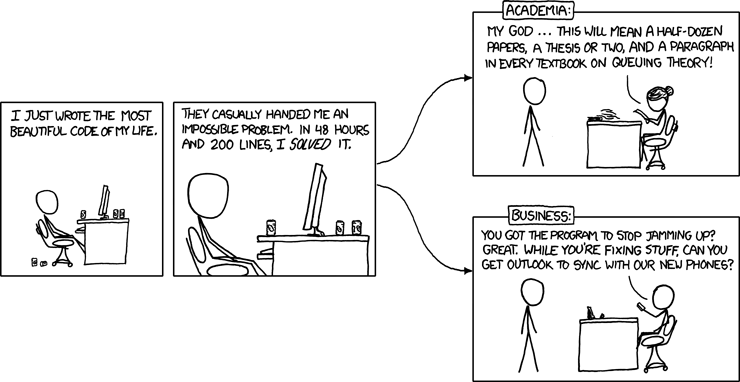
\includegraphics[scale=0.45]{images/academia_vs_business.png}
\\
\end{document}
